\label{Organisation}

\section{Schedule}

As with any software project, planning is an important aspect. As is to be expected from a group without much prior experience in team work, the original schedule was overly optimistic. Other course deadlines and a failure to appriciate the time requirements of each stage resulted in a failure to meet our planned deadlines. 

\begin{figure}[!h]
    \begin{center}
        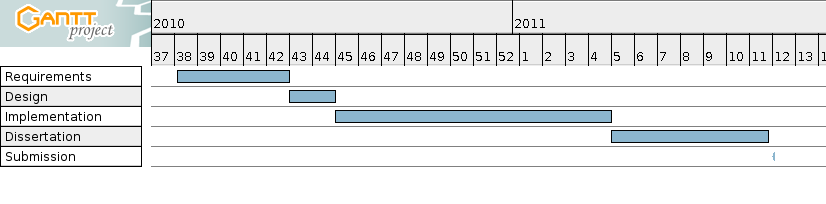
\includegraphics[width=14cm]{appendix/Diagrams/GIMplan.png}
        \caption{Gantt chart of our planned schedule.}
        \label{lockingDia}
    \end{center}
\end{figure}

\begin{table}[!h]
\begin{center}
\caption{Planned dates for each stage of the development process}
\begin{tabular}{ | p{4cm} |p{4cm}  |p{4cm} | } 
    \hline
    Reqirements & 21/09/10 & 25/10/10 \\
    \hline
    Design & 25/10/10 & 08/11/10 \\
    \hline
    Implementation & 08/11/10 & 31/01/11 \\
    \hline
    Dissertation & 31/01/11 & 20/03/11 \\
    \hline
\end{tabular}
\end{center}
\end{table}

\pagebreak

\begin{figure}[!h]
    \begin{center}
        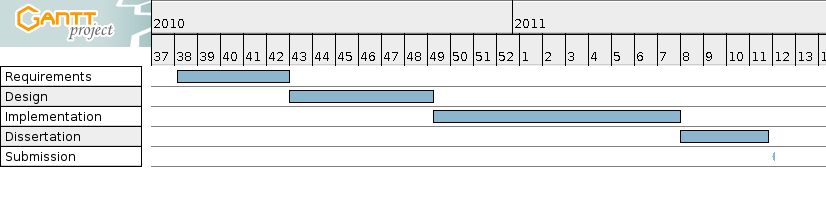
\includegraphics[width=14cm]{appendix/Diagrams/GIMreal.png}
        \caption{Gantt chart of our actual schedule.}
        \label{lockingDia}
    \end{center}
\end{figure}

\begin{table}[!h]
\begin{center}
\caption{Dates acheived during the development process}
\begin{tabular}{ | p{4cm} |p{4cm}  |p{4cm} | }
    \hline
    Reqirements & 21/09/10 & 25/10/10 \\
    \hline
    Design & 25/10/10 & 08/12/10 \\
    \hline
    Implementation & 08/12/10 & 21/02/11 \\
    \hline
    Dissertation & 21/02/11 & 20/03/11 \\
    \hline
\end{tabular}
\end{center}
\end{table}

The process of designing the system took far longer than was initially anticipated, which delayed the implementation process significantly. The implementation for basic functionality went smoothly and was finished relatively quickly, however a large amount of time was spent improving the interface and polishing the program. Our original plan provided almost 2 months to write this dissertation, in reality we had only 1 month.  

\section{Version Control}

For this project we used version control to manage code and documentation. All internal documentation was hosted using Google Docs, while this document and the java code was managed using SVN provided by Google Code. Our project initally used the SVN provided by the Computing Science school in Glasgow University, however, due to stability and relability issues we moved our project to Google's infrastructure.
